\documentclass[12pt]{article}\usepackage[]{graphicx}\usepackage[]{color}
%% maxwidth is the original width if it is less than linewidth
%% otherwise use linewidth (to make sure the graphics do not exceed the margin)
\makeatletter
\def\maxwidth{ %
  \ifdim\Gin@nat@width>\linewidth
    \linewidth
  \else
    \Gin@nat@width
  \fi
}
\makeatother

\definecolor{fgcolor}{rgb}{0.345, 0.345, 0.345}
\newcommand{\hlnum}[1]{\textcolor[rgb]{0.686,0.059,0.569}{#1}}%
\newcommand{\hlstr}[1]{\textcolor[rgb]{0.192,0.494,0.8}{#1}}%
\newcommand{\hlcom}[1]{\textcolor[rgb]{0.678,0.584,0.686}{\textit{#1}}}%
\newcommand{\hlopt}[1]{\textcolor[rgb]{0,0,0}{#1}}%
\newcommand{\hlstd}[1]{\textcolor[rgb]{0.345,0.345,0.345}{#1}}%
\newcommand{\hlkwa}[1]{\textcolor[rgb]{0.161,0.373,0.58}{\textbf{#1}}}%
\newcommand{\hlkwb}[1]{\textcolor[rgb]{0.69,0.353,0.396}{#1}}%
\newcommand{\hlkwc}[1]{\textcolor[rgb]{0.333,0.667,0.333}{#1}}%
\newcommand{\hlkwd}[1]{\textcolor[rgb]{0.737,0.353,0.396}{\textbf{#1}}}%
\let\hlipl\hlkwb

\usepackage{framed}
\makeatletter
\newenvironment{kframe}{%
 \def\at@end@of@kframe{}%
 \ifinner\ifhmode%
  \def\at@end@of@kframe{\end{minipage}}%
  \begin{minipage}{\columnwidth}%
 \fi\fi%
 \def\FrameCommand##1{\hskip\@totalleftmargin \hskip-\fboxsep
 \colorbox{shadecolor}{##1}\hskip-\fboxsep
     % There is no \\@totalrightmargin, so:
     \hskip-\linewidth \hskip-\@totalleftmargin \hskip\columnwidth}%
 \MakeFramed {\advance\hsize-\width
   \@totalleftmargin\z@ \linewidth\hsize
   \@setminipage}}%
 {\par\unskip\endMakeFramed%
 \at@end@of@kframe}
\makeatother

\definecolor{shadecolor}{rgb}{.97, .97, .97}
\definecolor{messagecolor}{rgb}{0, 0, 0}
\definecolor{warningcolor}{rgb}{1, 0, 1}
\definecolor{errorcolor}{rgb}{1, 0, 0}
\newenvironment{knitrout}{}{} % an empty environment to be redefined in TeX

\usepackage{alltt}
\usepackage{geometry}
\usepackage[round]{natbib}
\usepackage{graphicx}
\geometry{a4paper}
\usepackage[T1]{fontenc}
\usepackage[utf8]{inputenc}
\usepackage{authblk}
\usepackage[running]{lineno}
\usepackage{setspace}
\usepackage{amsfonts,amssymb,amsmath,graphicx,hyperref}
\doublespacing




%-------------------------------------------------------------------------

\title{Climate drivers of plant population extinction debt}

\author{Kevin Czachura}
\author{Tom E.X. Miller}
\affil{Program in Ecology and Evolutionary Biology, Department of BioSciences, Rice University, Houston, TX USA}
\renewcommand\Authands{ and }
\date{*Corresponding author: tom.miller@rice.edu}

%-------------------------------------------------------------------------
\IfFileExists{upquote.sty}{\usepackage{upquote}}{}
\begin{document}
\maketitle


%-------------------------------------------------------------------------
\section*{Summary}
\begin{enumerate}
  \item The background to the question (why it is interesting)
  \item What the question is
  \item What was done in the study
  \item What was found
  \item  What this means in the context of the broad field of animal ecology
   \ldots
   \end{enumerate}
   
%-------------------------------------------------------------------------
\section*{Keywords}
Listed in alphabetical order, the key-words should not exceed 10 words or short phrases. Please pay attention to the keywords you select: they should not already appear in the title or abstract. Rather, they should be selected to draw in readers from wider areas that might not otherwise pick up your paper when they are using search engines.

%--------------------------------------------------------------------
\section*{Introduction}
\linenumbers
Climate change has had a major impact around the globe, and the climate is projected to continue changing in the future (IPCC 2007). 
Moreover, ecological studies have found that climate change has the potential to cause massive change in Earth’s ecosystems in a short span of time (Walther et al. 2002). 
At the population level, long-term monitoring has suggested that the effects of climate change over the past century are already apparent (Hughes 2000). 
Thus, we should prioritize studies connecting long-term biological datasets to abiotic environmental drivers such as climate (Harrington et al. 1999). 
We can make this connection using the framework of population ecology.\\ \\

Demographic models are a useful tool for studying populations, and there are a number of methods to incorporate climate variables into them. 
Maschinski et al. (2006) simply categorized years as drought or non-drought in their demographic model of an endangered shrub in the Sonoran Desert. 
Dalgleish et al. (2011) compiled a list of climate variables that correlated with random effects of year for their three-year study of a sagebrush steppe species, then ran candidate models with different combinations of these short-listed climate models to find the best model.\\ \\

Demographic studies have found that the dynamics of a variety of different plant populations in various ecosystems have shown climate change responses (Dalgleish et al. 2011, Sletvold et al. 2013, Williams et al. 2015).
Sletvold et al. (2013) found that the growth rate of a population of orchids increased due to warmer summer temperatures, which increased the survival rate of individuals in the population. 
In another orchid species, Williams et al. (2015) found that different vital rates were affected by different climatic variables, but that number of flowers produced was reduced in warmer years. 
Climate has also been found to influence the population growth rate of three different plant species that dominate the landscape in the sagebrush steppe of Western North America (Dalgleish et al. 2011).\\ \\

Climate can also be linked to the population growth rate \(\lambda\), and there are a couple of ways to do this. 
In the past, matrix models have been widely used to understand population dynamics and inform population management, but there has been criticism that their results may not be entirely reliable (Crone et al. 2011). 
One suggestion Crone et al. (2011) has to make these models more reliable is to use more long-term datasets. 
Another method of understanding population dynamics is to use an integral projection model (IPM). 
An IPM is useful because it allows for structural traits to be continuous instead of arbitrarily discrete, and can incorporate more complex demographical traits (Ellner and Rees 2006). 
In this study, we approach our research questions using an IPM.\\ \\

Here we use demographic modeling with a 12-year set of data from a population of \textit{O. imbricata} to ask four questions regarding climate effects on this species: (1) Can climate variables explain some of the year-to-year variation in vital rates? (2) How does climate affect \(\lambda\), the population growth rate? (3) Given that recent \(\lambda\) indicates a population in decline, can we use historical climate data to determine the conditions under which \(\lambda\) $>$ 1? (4) What implications does climate change hold for the population?

%--------------------------------------------------------------------
\section*{Materials and methods}


\subsection*{Study site and demographic data collection}
The focal species \textit{Opuntia imbricata} Haw. [D.C.] (`tree cholla cactus') is widely distributed throughout desert and grassland habitats of the southwest U.S.
These long-lived (30-plus-year), CAM plants grow through the production and elongation of cyclindrical stem segments. These vegetative structures as well as flowerbuds are initiated in late spring. 
Flowering occurs in early summer and stem segment elongation takes place during the remainder of the growing season. 
We divide the calendar year into warm-season months (May through September), when vegetative growth and reproduction occur, and cool-season months (October through April).

This study was conducted at the Sevilleta National Wildlife Refuge (SNWR), a Long-Term Ecological Research (SEV-LTER) site in central New Mexico. 
Our focal population occurs in the Los Pinos mountains at an elevation of blank and give lat-long. 
Tree cholla are a dominant component of the vegetation in this area (give density), along with oaks, yucca, Pinon pine, and perennial grasses (\textit{Bouteloua gracilis} and \textit{B. eriopoda}).
The present study relies on long-term (2004--2017) demographic data on individual-level measures of growth (change in size, approximated as the volume of a cone based on height and width measurements), survival, and reproduction (number of flowerbuds) recorded from tagged plants in late May or early June of each year, a pre-breeding census. 
We treat May 1 as the start of the transition year (coincident with the start of the warm-season months).
There are a total of 1150 unique individuals in the data set and 5803 transition-year observations from 4--8 plots or spatial blocks depending on the year. 
Full details of the study design and data collection are given elsewhere (cite Compagnoni, Ohm, Miller and Elderd).

\subsection*{Climate data}

Our goal was to connect inter-annual variation in demography to corresponding variation in climate.
SEV-LTER collects climate data from a network of meteorolgical stations throughout SNWR, with the oldest records coming from the late 1980s.
While the SEV-LTER climate data cover years of our plant demographic data collection, our intention was to ``back-cast" demographic performance farther back into the 20th century. 
We therefore gathered climate data from ClimateWNA v5.60 \citep{wang2016locally}, a software package that uses PRISM \cite{daly_physiographically_2008} and WorldClim \cite{hijmans_very_2005} data to calculate downscaled data for western North America based on location and elevation, going back as far back as 1900.
By relying on downscaled, interpolated climate data instead of direct observations from meteorological stations, we knew that we were trading off local resolution in favor of more historical years of data.
We quantified this loss of resolution by comparing predictions from ClimateWNA to SEV-LTER data for years that they over-lapped (give years), with downscaled data based on the lat-long (give) and elevation (give) of the SEV-LTER meteorological station that was nearsest our study population (station ID 50, ca. 2 km from our study sites).
We found that the two data sets were highly correlated (Appendix), which bolstered our confidence that ClimateWNA provided locally accurate climate data for both the demographic observation period as well as historical years that preceded our study.

We derived seasonal estimates (warm-season and cool-season) of total precipitation and mean, minimum, and maximum temperature from monthly climate data, for a total of eight variables. Months were aligned to correspond to demographic transition years rather than calendar years, which means the cool-season climate for a transition year beginning in May of calendar year $t$ spans October of year $t$ through April of year $t+1$. 

To reduce the dimensionality of the climate data, we conducted Principal Component Analysis (PCA) on the eight climate variables (two seasons x four variables) for the years 1900-2017, with climate values scaled to unit variance. We used the prcomp() function in R version to estimate variance in the climate data explained by each PC and variable loadings, which give the correlations between original variables and PC values.

\subsection*{Statistical modeling}


%We built generalized linear mixed models (GLMM) in a hierarchical Bayesian framework to connect inter-annual demographic variability to climate drivers, as capture by three PCs that collectively explained var_explained\% of the inter-annual variation in climate.

\subsection*{Demographic modeling}

%--------------------------------------------------------------------
\section*{Results}

\begin{figure}[h!]
  \label{fig:PCA}
\begin{knitrout}
\definecolor{shadecolor}{rgb}{0.969, 0.969, 0.969}\color{fgcolor}

{\centering 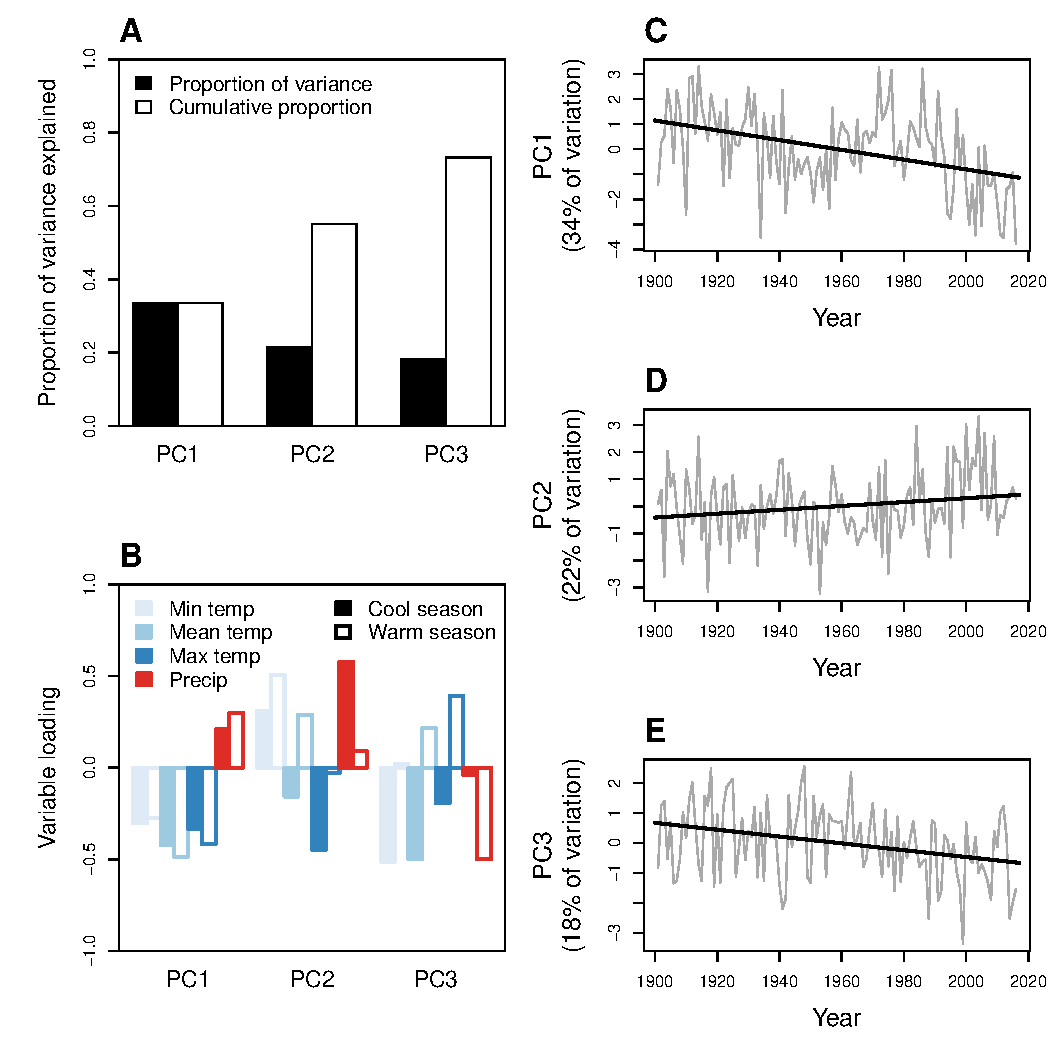
\includegraphics[width=\maxwidth]{figure/PCA_results-1} 

}



\end{knitrout}
  \caption{Principal component analysis (PCA) of eight seasonal climate variables for demographic transition years (May 1 -- April 30) of 1901 through 2016. 
  (A) Variance and cumulative variance explained by first three principal components. 
  (B) Loadings of original variables onto PC axes. Loading values can be interpreted as correlations between each raw variable and each PC. 
  (C--E) Temporal trends in climate; PC values shown in grey and regression lines shown in black. 
  PC1: $F_{1,114} = 21.72$, $P < 0.001$; 
  PC2: $F_{1,114} = 3.98$, $P < 0.05$; 
  PC3: $F_{1,114} = 12.77$, $P < 0.001$.}
\end{figure}

\newpage
\begin{figure}[h!]
  \caption{}
  \label{Fig1}
  \begin{center}
    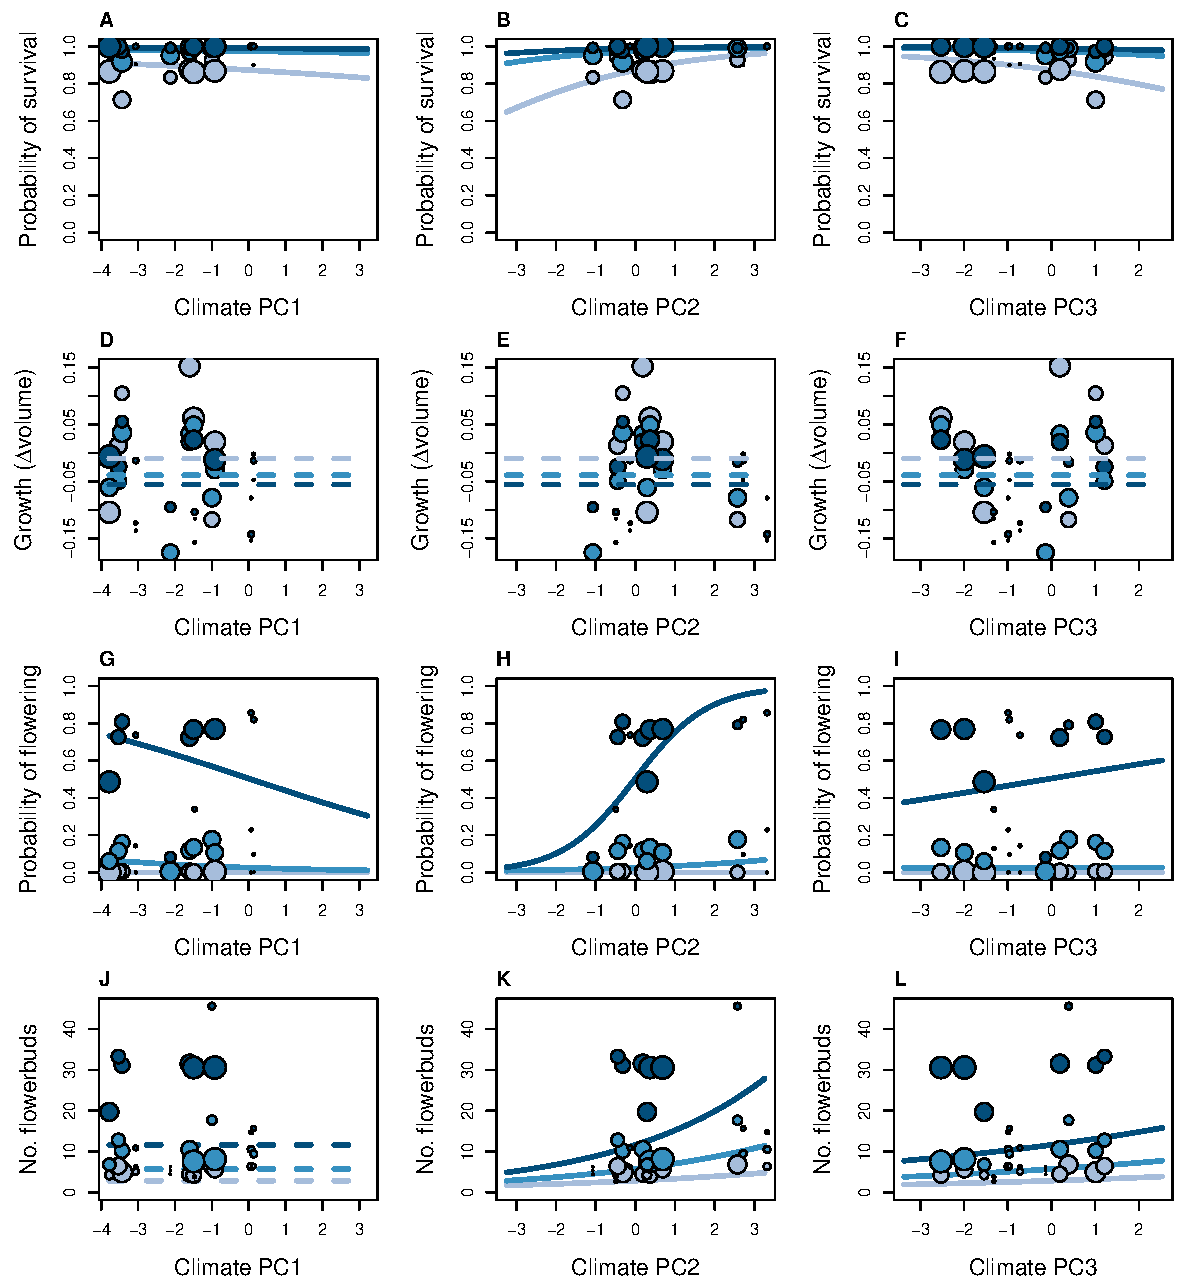
\includegraphics[width=\linewidth]{Figures/vital_rates.pdf}
  \end{center}
\end{figure}


%--------------------------------------------------------------------
\section*{Discussion}

%--------------------------------------------------------------------
\section*{Acknowledgements}

%--------------------------------------------------------------------
\section*{Data accessiblity}

\bibliographystyle{jae}%Compile with jae.bst style file
\bibliography{cholla_climate}

%--------------------------------------------------------------------
\newpage
\section*{Appendix A: Correspondence between downscaled and locally measured climate variables}
\renewcommand{\thefigure}{A\arabic{figure}}\setcounter{figure}{0}
\renewcommand{\thetable}{A\arabic{table}}\setcounter{table}{0}


We compared warm- and cool-season values of four climate variables (total precipitation and minimum, mean, and maximum temperature) between two data sources: the SEV-LTER meteorological station nearest our study site (station 50 in the SEV-LTER meteorological network) and downscaled data from ClimateWNA corresponding to the same latitude, longitude, and elevation as station 50. Our goal was to determine how well the downscaled data captured conditions `on the ground' as measured directly by the meteorological station. We compared the years 2001 through 2017, which are the years of overlap between the two data sources.

There was strong agreement between the two data sources, with statistically significant positive correlations (at $\alpha = 0.1$) for nearly all variables (Table \ref{tab:WNASEV}, Figure \ref{fig:WNASEV}). Temperature extrema were less strongly correlated between the two data sets than temperature means, which is unsurprisingly given that extreme values may be sensitive to local micro-environmental conditions that the relatively coarse downscaled data would miss. The weakest correlation was that of warm-season temperature (Spearman's $r = 0.41$, $P = 0.11$). 

\newpage
\begin{table}[h!]
  \caption{Correlations between seasonal climate values measured by an on-site meteorological station versus dowwscaled data from ClimateWNA corresponding to the same years and location. Correlation values show Pearson correlations and P-values come from $t$-tests with 14 degrees of freedom. Gray lines show $y=x$.}
  \label{tab:WNASEV}
  \begin{center}
    \begin{tabular}{p{2cm}p{5cm}p{2cm}p{2cm}}
      \hline
      Season & Variable & Correlation & P-value\\
      \hline
      Warm & Min temperature & 0.59 & 0.0153 \\
      Warm & Mean temperature & 0.84 & \ensuremath{10^{-4}} \\
      Warm & Max temperature & 0.41 & 0.1135 \\
      Warm & Precipitation & 0.49 & 0.0544 \\
      
      Cool & Min temperature & 0.51 & 0.0622 \\
      Cool & Mean temperature & 0.94 & 0 \\
      Cool & Max temperature & 0.69 & 0.0069 \\
      Cool & Precipitation & 0.87 & 0 \\
      \hline
    \end{tabular}
  \end{center}
\end{table}

\begin{figure}[h!]
  \caption{Correlations between seasonal climate values between SEV-LTER metereological data and downscaled estimates from ClimateWNA for years 2001--2017.}
  \label{fig:WNASEV}
\begin{knitrout}
\definecolor{shadecolor}{rgb}{0.969, 0.969, 0.969}\color{fgcolor}

{\centering 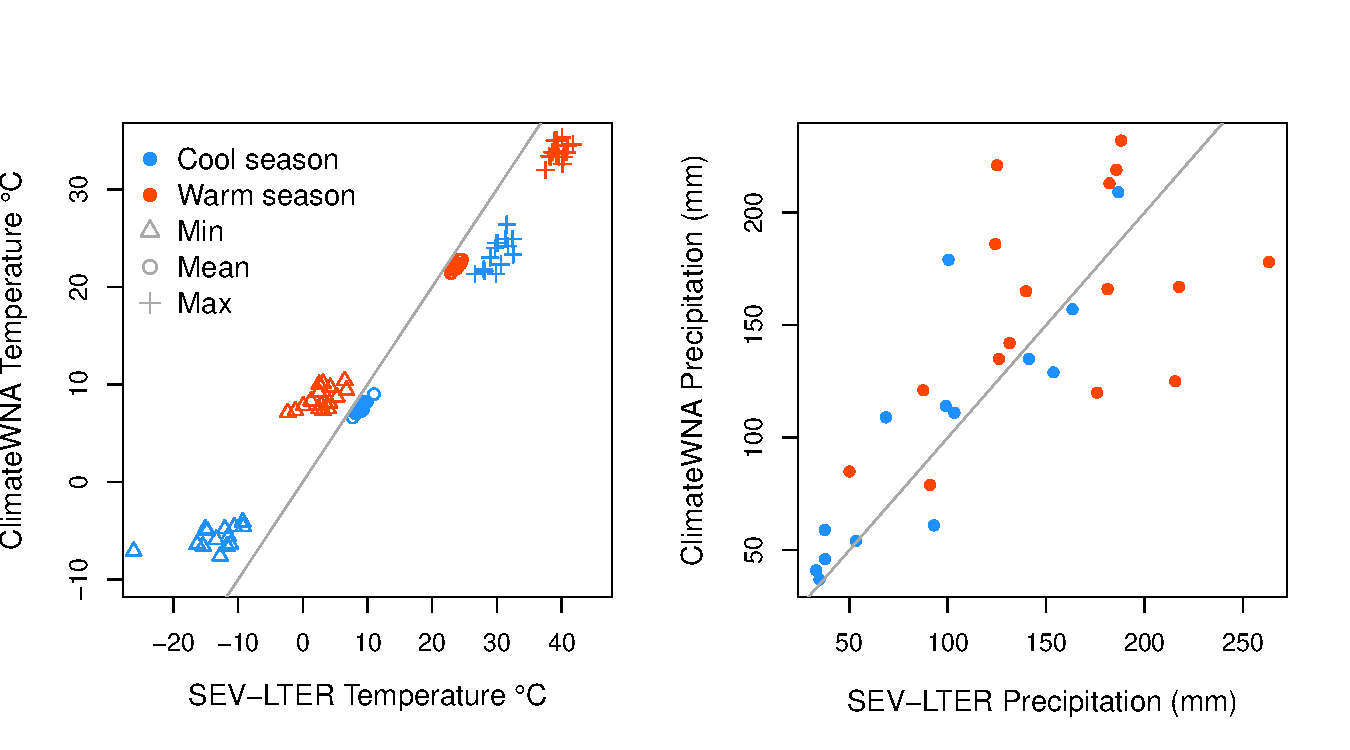
\includegraphics[width=\maxwidth]{figure/SEV_WNA_corr-1} 

}



\end{knitrout}
\end{figure}

%--------------------------------------------------------------------
\newpage
\section*{Appendix B: Vital rate modeling and stochastic variable selection}

We fit generalized linear mixed effects models in a hierarchical Bayesian statistical framework to quantify climate dependence in demographic vital rates. 
There were four size-dependent vital rates, measured in the long-term study, for which we could additionally estimate climate dependence: survival from year \textit{t} to year \textit{t+1}, individual growth (change in size from year \textit{t} to year \textit{t+1}), probability of flowering, and the number of flowerbuds produced, given that a plant flowered. 
All of the vital rate models used the same general linear predictor for the expected value ($\mu$) but apply a different link function ($f(\mu)$) depending on the distribution of the observations:
\begin{align}\label{eq:VR_lin_pred}
\begin{split} 
f(\mu) = \beta_{0} + \beta_{1}x + \\ 
\rho^{1}_{1}PC1 + \rho^{1}_{2}PC1^{2} + \rho^{1}_{3}xPC1 + \rho^{1}_{4}xPC1^{2} + \\
\rho^{2}_{1}PC2 + \rho^{2}_{2}PC2^{2} + \rho^{2}_{3}xPC2 + \rho^{2}_{4}xPC2^{2} + \\
\rho^{3}_{1}PC3 + \rho^{3}_{2}PC3^{2} + \rho^{3}_{3}xPC3 + \rho^{3}_{4}xPC3^{2} + \\
\gamma + \tau
\end{split}
\end{align}
The linear predictor includes a grand mean intercept ($\beta_{0}$) and size-dependent slope ($\beta_{1}$). The size variable $x$ is the natural logarithm of plant volume ($log_{e}(cm^{3})$), which was standardized to mean zero and unit variance for analysis. Other fixed-effect coefficient ($\rho$) correspond to climate variables and climate $\times$ size interactions. The climate variables are the three principal components ($PC1$, $PC2$, $PC3$) of inter-annual variation in temperature and precipitation. We include quadratic terms for climate to account for the possibility of non-monotonic climate responses. Climate coeffificient ($\rho$) superscripts correspond to each PC, and subscripts correspond to linear, quadratic, and size-interaction effects. Finally, the linear predictor includes normally distributed random effects for plot-to-plot variation ($\gamma \sim N(0,\sigma_{plot})$) and year-to-year variation that is unrelated to climate effects captured by PCs 1-3 ($\tau \sim N(0,\sigma_{year})$).

\subsection*{Stochastic variable selection}

Because we intended to extrapolate the vital rate models into past climate environments that were not well represented during the long-term study, it was important that we simplify the vital rate models to exclude unnecessary coefficients (which, even if small in absolute value, could generate unrealistic predictions when extrapolated over a greater range of climate than the models were fitted to). To do this, we used stochastic variable selection, a `model-based model selection' approach \citep{hooten2015guide} that generates weightings for each fixed-effect coefficient, indicating the probability that the coefficient is non-zero. We employed an approach based on George and McCulloch (\citeyear{george1993variable}) where each coefficient ($C_{i}$) is modeled as a mixture distribution with zero and non-zero modes, where modal frequency is determined by an indicator variable ($z_i$). The coefficient prior was:
\begin{align}\label{eq:SVS}
C_i \sim (1-z_i) * N(0,0.1) + z_i * N(0,1000) \\
z_i \sim Bernoulli(0.5)
\end{align}
The first term of the mixture distribution assigns, with probability $(1-z_i)$, a prior with mean zero and arbitrarily small variance, effectively forcing the posterior estimate to equal zero. The second term assigns, with probability $z_i$, a prior with mean zero and arbitrarily large variance, which allows for a non-zero posterior estimate. The posterior distribution of the indicator variable $z_i$ gives the probability that the coefficient is non-zero. We estimated this probability for each coefficient in Eq. \ref{eq:SVS} and retained in the final model all coefficients with a posterior mean $\hat{z_i} > 0.1$, meaning that the model term is assumed to be zero with 90\% confidence. All $z_i$ values from the full model are shown in Table \ref{tab:SVS}.

% latex table generated in R 3.4.0 by xtable 1.8-2 package
% Tue Dec 11 10:32:59 2018
\begin{table}[ht]
\centering
\begin{tabular}{rlllll}
  \hline
Climate PC & Model term & Survival & Growth & Flowering & Fertility \\ 
  \hline
 & Size & $\mathbf{1}$ & $\mathbf{0.53}$ & $\mathbf{1}$ & $\mathbf{1}$ \\ 
    1 & PC & $\mathbf{0.13}$ & 0.04 & $\mathbf{0.12}$ & 0.05 \\ 
    1 & PC*PC & 0.03 & 0.01 & 0.03 & 0.01 \\ 
    1 & PC*size & 0.06 & 0.01 & 0.08 & 0.07 \\ 
    2 & PC & $\mathbf{0.18}$ & 0.03 & $\mathbf{0.11}$ & $\mathbf{0.14}$ \\ 
    2 & PC*PC & 0.06 & 0.01 & 0.06 & 0.03 \\ 
    2 & PC*size & 0.04 & 0.02 & $\mathbf{1}$ & $\mathbf{0.27}$ \\ 
    3 & PC & $\mathbf{0.18}$ & 0.02 & $\mathbf{0.12}$ & $\mathbf{0.18}$ \\ 
    3 & PC*PC & 0.09 & 0.01 & 0.09 & 0.06 \\ 
    3 & PC*size & 0.06 & 0.01 & $\mathbf{0.13}$ & 0.03 \\ 
   \hline
\end{tabular}
\caption{Stochastic variable selection results. Bolded values indicate terms retained in the final model.} 
\label{tab:SVS}
\end{table}



%--------------------------------------------------------------------
\newpage
\section*{Appendix C: Assembling life cycle components into an IPM}

\end{document}
